\documentclass[a4paper]{article}
\usepackage[utf8]{inputenc}

\usepackage{graphicx, url}

\usepackage{amsmath, amsfonts, amssymb, amsthm}
\usepackage{xfrac, mathptmx}

\newcommand{\obj}[1]{{\left\{ #1 \right \}}}
\newcommand{\clo}[1]{{\left [ #1 \right ]}}
\newcommand{\clop}[1]{{\left [ #1 \right )}}
\newcommand{\ploc}[1]{{\left ( #1 \right ]}}

\newcommand{\brac}[1]{{\left ( #1 \right )}}
\newcommand{\induc}[1]{{\left . #1 \right \vert}}
\newcommand{\abs}[1]{{\left | #1 \right |}}
\newcommand{\nrm}[1]{{\left\| #1 \right \|}}
\newcommand{\brkt}[1]{{\left\langle #1 \right\rangle}}
\newcommand{\floor}[1]{{\left\lfloor #1 \right\rfloor}}

\newcommand{\Real}{\mathbb{R}}
\newcommand{\Cplx}{\mathbb{C}}
\newcommand{\Pwr}{\mathcal{P}}

\newcommand{\defn}{\mathop{\overset{\Delta}{=}}\nolimits}

\usepackage[russian, english]{babel}
\newcommand{\eng}[1]{\foreignlanguage{english}{#1}}
\newcommand{\rus}[1]{\foreignlanguage{russian}{#1}}

\title{Computer lingusitics}
\author{Nazarov Ivan, \rus{101мНОД(ИССА)}\\the DataScience Collective}
\begin{document}
\selectlanguage{english}
\maketitle

\selectlanguage{russian}
\section{Лекция \#1} % (fold)
\label{sec:lecture_1}
\eng{2015-01-12: Introduction}
\begin{enumerate}
	\item Практические мелкие задачи -- поверхностный синтаксический анализ
	\item Работоспособное приложение
	\item Теория
\end{enumerate}
\eng{Natural Language Processing}
\eng{Computaional linguistics}
Общая лингвистика \begin{itemize}
	\item Синтаксис, синтактика
	\item Семантика
	\item Прагматика -- естественный язык со своими особенностями развивался из соображений удобства решения пракитических задач гоминидов.
\end{itemize}	
Теория формальных языков, Иерархия грамматик Хомского (\eng{Noam Chomsky})

\eng{Quatitative (statistical) linguistics}

Проблема существования языковой универсали (инвариант):
к сожалению среди всех языков универсалью может лищь считаться существование гласных и согласных.
Среди европейских языков -- существование частей речи.

Семиотика -- теория знаковых систем.
Треугольник Фреге
\begin{description}
	\item[\eng{Signifier}] Смысловой символ
	\item[\eng{Signified}] Представление в сознании
	\item[\eng{Referent}] Целевой предмет или явление
\end{description}

Базовые единицы:
\begin{itemize}
	\item фонемы/графемы
	\item лексемы
\end{itemize}

Уровни:
\begin{itemize}
	\item Синтаксичечкий -- предложение
		словосочетания $\to$ сверхфразовые единства
	\item Графематический -- графемы
	\item Морфологический -- слова
	\item Семантический -- элементарная единица ``сема''
	\item Дискурсивный -- \eng{Coherent connected set of sentences}
\end{itemize}

Невозможность взаимо однозначного отображения лексемы в смысл
\begin{description}
	\item[Полисемия] многозначность языковой единицы
	\item[Синонимия] совпадение единиц по смыслу
	\item[Омонимия] совпадение единиц по форме, существенное различие по смыслу.
	Бывает лексическая и морфологическая.
\end{description}

\begin{itemize}
	\item Семантические сети
	\item Синтез нового текста -- языковая компетенция
	\item векторная модлеь текста (\eng{bag of words})
\end{itemize}

% section lecture_1 (end)

\selectlanguage{russian}
\section{Лекция \# 2} % (fold)
\label{sec:lecture_2}

Вычислительная (квантитативная) лингвистика опирается на предположение, что то, что верно для выборки текстов, верно для всей совокупности текстов и даже для всего естественного языка в целом (возможно имеется ввиду репрезентативная выборка).

Для каждой статистической единицы текста подсчитывается число употреблений в тексте (группе текстов) $T$:
для каждого объекта $e\in \mathcal{E}$ абсолютная частота
\[a_e \defn \#\obj{\text{вхождение сущности } e \text{ в текст } T}\]

Относительная частота отражает частотные характеристики внутри одного текста (группы текстов) $T$.
Для объекта $e\in \mathcal{E}$ \[r_e \defn \frac{a_e}{\#\text{различные сущности в } T}\]

Возможные \textbf{статистические сущности} перечислены ниже:
\begin{description}
	\item[Лемма (Слово)] \hfill\\
	Слово в широком смысле -- единица морфологического анализа, единица толкового словаря, каноническая, основная, начальная форма словоформы (сохранение части речи, аспекта, времеи и т.п.).
	\item[Словоформа] \hfill\\
	Слово в узком смысле -- одинаковая последовательность фонем. Совокупность словоформ одной лексемы -- слвоизменительная парадигма.
	\item[Словоупотребление] \hfill\\
	Вхождение словоформы в текст, единица текста.
\end{description}

При подсчёте статистики символов нужно всегда понимать, показательная ли она.
Частоты символов ($n$-грамм):
\begin{description}
	\item[относительная] \hfill\\
	частота на уникальный символ (внутри одного текста);
	\item[абсолютная] \hfill\\
	частота на все символы (между текстами).
\end{description}

Общая форма гистограммы абсолютных частот букв сохраняется от текста к тексту -- характеристика языка. Может использоваться для:
\begin{description}
	\item[Определение кодировки текста]\hfill\\
	при верном определении количество недопустимых биграмм минимально;
	\item[Определение языка текста] \hfill\\
	Единица \eng{Schilling}
	\item[Определение схожести текстов]
	\item[Дешифровка текстов] \hfill\\
	В случае простоых перестановочных шифров.
\end{description}


% \eng{Brown's corpus}

\begin{description}
	\item[Закон Ципфа (\eng{Zipf's law})] \hfill\\
	Текст $\to$ Частотный список слов $\to$ Частота слова обратно пропорциональна рангу слова $\to$ Распределение с тяжёлым хвостом $\to$ соотношение Парето:
	``Большая часть текста формируется минимальными количеством слов.''
	Эмпирический закон, имеет недостатки:
	\begin{itemize}
		\item Художественный текст лексически богаче, чем технический.
		\item Нарушается на фрагментах текста $\implies$ закон не языка, а текста.
		\item проверка текста на естественность (зная тему, можно сравнить с эталоном).
	\end{itemize}


	\item[Формула Кондона] \hfill\\
	Для относительных и абсолютных частот при переходе к \eng{log-log} шкале прослеживается линенйная зависимость. Исходя из этого степенной закон распределения Ципфа обощается до одыкновенного \eng{Power law}:
	\[a_e \defn \frac{C}{\text{rank}_e^\gamma}\,\text{ и }\,r_e \defn \frac{C}{N \text{rank}_e^\gamma}\]
	где $N$ -- общее количество словоупотреблений в тексте,
	$\gamma>0$ -- коэффициент лексического богатстсва текста, зависящий от тектста, автора, стиля, направленности и т.п.
	Эмпирически выясняется, что мем меньше $\gamma$ тем богаче язык по словоформам.

	\item[\eng{Zipf-Mandelbr\:ot law}] \hfill\\
	Кодирование сообщений. Чем чаще слово тем короче код. Можно наблюдать в естественном языке: служебные слова, например. (Хаффман). В процессе развития естественный язык самооптимизировался.

	Для малых рангов (более частых слов) закон Ципфа нарушается. Вводится поправка для высокочастотных статистических единиц:
	\[a_e \defn \frac{k N}{\brac{\rho + \text{rank}_e}^\gamma}\]
	\begin{itemize}
		\item Плохо работает на очень редких словах (тяжёлый хвост).
		\item Константы зависят от стиля и длины
		\item Постоянство $\gamma$ не сохраняется.
		\item Даёт лишь грубое приближение к статистической структуре текста.
	\end{itemize}

	\item[\eng{Herdan-Heaps law}] \hfill\\
	Эмпирический закон, согласно которому количество различных слов (?) увеличивается с ростом объёма текста с убывающей отдачей:
	\[V(N)\defn K N^\beta\]
	То есть с ростом объёма текста не происходит насыщения словаря уникальных слов, из которого состоит текст, однако скорость выявления словаря убывает. 
\end{description}

Стоп-список для несмысловых слов.
Выявление наиболее значимых слов -- они имеют среднюю частоту.
Средняя длина слова также может играть роль в определении определение стиля/темы/автора.

$n$\eng{-gramm} модель.
Рассмотрим $W = \brac{w_i}_{i=1}^n$ -- некоторая $n$-грамма.
Предполагается, что вероятность сущности текста зависит от предыдущих $n-1$ сущностей.
\[ \Pr(W) = \Pr\brac{w_1,w_2,\ldots,w_n} = \prod_{k=1}^n \Pr\brac{\induc{w_k}\,\brac{w_i}_{i=1}^{k-1}}\]
Вероятность всего предложения вычисляется как произведение вероятности всех входящих в него $n$-грамм.

Разложение совместной вероятности в предположении направленности порядка слов позволяет строить модели, способные синтезировать текст:

На практике объём корпуса ограничен (и есть закон Хердана-Хиппса), то не все $n$-граммы представлены.
Поэтому можно ввести упрощение вероятности $n$-граммы до марковской цепи порядка $k\leq n-1$:
\[\Pr\brac{w_1,w_2,\ldots,w_n} = \prod_{j=1}^n \Pr\brac{\induc{w_j}\,\brac{w_{j-i}}_{i=1}^k}\]

Изложенная модель проста и легко строится по любому корпусу.
Однако требует колоссального объёма информации, поскольку \eng{scope} корпуса ограничен,
то нет возможности определить допустима или нет отсутствующая $n$-грамма (её вероятность $0$).

Сглаживание -- повышение вероятности одних $n$-грамм за счёт других.
Пример для биграмм : \[\Pr\brac{\induc{w_2}\, w_1} = \frac{r_{w_1w_2}+\alpha}{r_{w_1}+\alpha V}\]
где $V$ -- количество единиц в тексте.

Коэффициент неопределённости (?)

% Домашка см лекция~2 слайд~50

% section lecture_2 (end)

\section{Лекция \# 3} % (fold)
\label{sec:lecture_3}

Корпусная лингвистика занимается теорией и практикой создания размеченных языковых корпусов.

Наличие разметки исследуемых целевых языковых явлений

Корпус и коллекция текстов отличаются тем, что в коллекции нет качеств охвата, полноты разметки, а главное цели собранных языковых явлений.

Лингвистические задачи: язык вид речи, стиль жанр, употребление слова, буквы, словосочетания, части речи и тп для анализа состояния языка пространственно (диалекты -- география) и/или во времени (изменчивость).

Корпус -- соответствие лингвистической задаче, должен быть репрезентативен, сбалансированный и без перекосов. Полнота охвата изучаемого явления. Массив данных с разметкой

Типы корпусов: \begin{itemize}
	\item Язык и параллельность многоязычных текстов
	\item Стиль жанр: публицистический, литературный и тп
	\item Полные или фрагментированные тексты
	\item Вид данных: речь, письмо
	\item Размеченные/неразмеченный
	\item Динамичность относительно пополнения
\end{itemize}
% RuWac, Генеральный корпус русского языка

Проблемы с корпусами:
\begin{itemize}
	\item Определить критерий отбора текстов
	\item решить проблемы с авторскими правами
	\item балансировка и репрезентативность
	\item приведение к единому формату текста и разметки
	\item сам процесс разметки
\end{itemize}

Поэтому корпусы создаются очень медленно и, зачастую, некачественно.
Корпусы не всегда масштабируемы на весь естественный язык: что норма в них, не всегда норма в языке.
Плохо отражает редкие явления.

%% В приложениях используются методы численной оптимизации.

Интернет не корпус, нет лингвистически релевантной разметки.
Плохо структурирован для задач лингвистических исследований.
Очистка от рекламы, меню контекстных/неконтекстных ссылок.

Корпуса всё-таки нужны, поскольку они могут служить эталонами.
Используются для построения статистических языковых моделей.

Берём слово для исследования частоты использования:
% многозначное или значимое изменение со временем
% написать отчёт о сходстве/различии
% Супруги -- парная конная упряжь

Исследование морфологических анализаторов русского языка, стемминг (откидывание словоизменительной части).
% solarix.ru
%% НКРЯ

%% Доклад на 2015-02-09 :
%% Байесовская вероятность и её использование


Морфологический (графематический) анализ очень важен!
% два направления: анализ текста и синтез текста

Графематический
Морфологический
	Приведение слова к нормальному виду слова (лемма), выделение основы слова (стемминг).
Постморфологический

Синтаксический
Семантический и прагматический

уровень символы и знаки текста
Графема -- минимальные неделимые единицы текста
Посимвольная обработка: выделение единиц \eng{tokenization}

\eng{Token} -- цепочка знаков от разделителя, до разделителя (пробелы, знаки препинания), соответствует лексеме в языках программирования.

\eng{Tokenization} -- Вычленение значимых единиц.

\begin{itemize}
	\item Слова могут быть написаны с ``разрядкой''
	\item преобразование числительных в числа
	\item восстановление правильного регистра (\eng{truecase})
	\item различия дефиса, тире и переноса: либо собрать слово, либо разделить на морфы
	\item нормализация сокращений
	\item свёртка составных предлогов или союзов, устойчивых фразеологизмов
	\item выделение полного имени (ФИО)
\end{itemize}
Для всего этого нужны словари сущностей.

Сложности
\begin{itemize}
	\item Неуниверсальности:
	\begin{itemize}
		\item Маркеры конца предложения (точка, троеточие, вопросительный или восклицательный знак)
		\item Маркеры начала предложения
	\end{itemize}
	\item пропуски знаков препинания (нужны контекст маркеры)
	\item оформление цитат, прямой речи
\end{itemize}

По размеченным текстам (в корпусе)
Инженерный подход \eng{rule-based}
\begin{itemize}
	\item словари имён, сокращений словосочетаний
	\item эвристические правила
\end{itemize}

Точность сегментации зависит от тематики, жанра.
Графематика почти никогда не идёт отдельно от морфологии

Инженерный подход: \url{http://aot.ru} -- вход текст, выход текст с дескрипторами, (основные, контекстные и макросинтактические).

% MyStem: нет морфологии если поток символов не разбит на единицы

Анализаторы основываются на регулярных грамматиках (\eng{Chomsky type 3}).

% section lecture_3 (end)

\section{Лекция \# 5} % (fold)
\label{sec:lecture_5}

Морфология

Морфосинтаксис
	словоизменительный класс
	лемма
	лексема
	особенности русской морфологии

Морфологические процессоры

морфемика -- внутренняя структура слова.

Как раздел лингвистики -- уровень слов
морфы объединяются в классы по смысловой инвариантности

Морфосинтаксис -- изменение склонение морфем в тексте.
морфологическое и синтаксическое выражение одной и той же мысли

% В русском языке есть упрощение 

Морфология кодирование смысла и грамматических признаков

Словоизменение
словобразование (добавление или изменение с помощью морфа)

``Слово -- строка'' неправильное определение слова.

с синтаксической точки зрения -- единицы текста
не обязательно выделяются пробелами
иогут включать небуквенные символы


Морфема -- минимальная значащая единица текста

в словах текста -- морфы
в языке -- морфемы

Алломорф -- разновидность морфа в словах

язык -- система знаков, текст -- реализация языка

виды морфов :
\begin{description}
	\item[Корень] носитель основного компонента значения;
	\item[Аффикс] префикс (приставка), суффикс, флексия (окончание), постфикс (частица) -- добавляют дополнительный смысл
\end{description}
Кореней много, а аффиксов не много.

Деривация -- добавление морфов
словосложение (\eng{compund})

Морфотактика -- правила формирования слова из морфов

Суффиксы чаще, чем префиксы

Отличие аффикса от корня -- нечёткий дополнительный смысл

словообразование
\begin{description}
	\item[Фонетическое] Изменением звука, сдвиг ударения;
	\item[Супплетевизм] Давно возникшие слова (идиоматичны);
	\item[Клитика] Слово без ударения, синтаксически отдельное слово, но фонетически реализуется как аффикс.
\end{description}

Разбиение слова на слоги по морфам
Лемматизация и стемминг

Изменения слов в структуре предложения

Части речи (\eng{Parts of speech})
Знаменательные (наречие ,прилагательное, глаголы, числительные)
служебные слова предлог союз частица


Слово в тексте нет, есть словоформа -- конкретная грамматическая форма
Лексем -- совокупность всех словоформ с одинаковым смыслом (единица словаря).
Лемма -- нормальная (базовая, каноническая) словарная форма лексемы,
Основа слова -- часть слова без окончания (stem)
Псевдооснова -- неизменяемая основная часть слова

Слайд~13
Морфологические параметры есть то, от чего завися словоформы

\begin{description}
	\item[Связанные] присущие лексеме в целом;
	\item[Свободные] различимы в разных словоформах лексемы
\end{description}

Морфологическая или словоизменительная парадигма.

Слвоизменительный класс -- слова с одинаковой слвоизменительной парадигмой

Дефектная парадигма -- что-то должно быть, а нет

Модели бывают разные (статистическая)

\eng{Stemming} -- 

Алгоритм Портера быстр для ангилйского и модифицирован для других языков

% section lecture_5 (end)

\section{Лекция \# 6} % (fold)
\label{sec:lecture_6}

Синтаксические анализаторы. единицы обработки -- предложения

на входе результат (пост-) морфологического анализа

приложения: машинный перевод, коррекция аннотирования, и тп

Сложность: предложение выражет законченную мысль -- предикативность, сложность формализации ЕЯ.

Структтура прдлоения и связи между ними.

Теория членов предложения неполна.
Виды связи: подчинительная и взаимоподчинительная. Необходимость формализации полдлежащих и тп.

Глагол -- корень синтаксического дерева; только одна связь -- подчинительная объект-субъект.

Отношение вложения между составляющими (\eng{constituents}).

Предложение -- цепочка словоформ $S = w_1, w_2, \ldots, w_n$. Составляющая -- это отрезок цепочки.

Проективность $\forall \alpha, \beta, \gamma \in S$ таких что $\alpha\to \beta$ ($\beta$ подчиняется $\alpha$) и в предложении $\gamma$ стоит между $\alpha$ и $\beta$, то $\alpha\to\gamma$.

%% Неканоничный магистр Йода

% section lecture_6 (end)

\section{Лекция \# 7} % (fold)
\label{sec:lecture_7}

Грамматические методы синтаксического анализа
Контекстно-свободные грамматика встроенная в парсер
\eng{ATN} -- \eng{Augmented Transition Network}
.

% section lecture_7 (end)

\section{Review} % (fold)
\label{sec:review}
\begin{enumerate}
	\item С какими научными дисциплинами связана область компьютерной лингвистики?\hfill\\
	общая лингвистика (морфология, синтаксис, семантика, лексикография), математика (теория формальнфых языков и грамматик, статистическая лингвистика), информатика (трансляция языков программирования), искуственный интеллект

	\item Перечислите основные отличия естественных языков от искусственных.\hfill\\
	сложная система возникщая в процессе человеческой деятельности, изменявшаяся исходя из прагматики языка как средства коммунмкации познания и мышления. Основне отличия -- открытость и изменчивость, нестандартная сочетаемость, избыточность, многознаячность или неопределённость слов. В процессе развития естественны язык самооптимизировался.

	\item В чем суть явления полисемии? омонимии? Приведите примеры.\hfill\\
	Полисемия -- множественность смысла языковой едницы; синонимия -- совпадение языковых единиц по основному смыслу (разлиие в оттенках иили силе); омонимия -- звуковое или письменное совпадение единиц без смысловой связи между единицами (лексческая, морфологическая, синтаксическая)

	\item Перечислите основные уровни (подсистемы) языковой системы.\hfill\\ \begin{itemize}
		\item графематический -- препроцессинг, разбиение текста на единицы, посимвольная обработка, классификация на основные единцы текста;
		\item морфологиеский -- отображение словоформ в лексемы (лемматизация и стемминг);
		\item постморфологический -- разрешение омонимии;
		\item (пред)синтактический -- сегментация на предложения и словосочетания, определение синтаксических групп, а также и ролей и подчинительных и сочинительных отношений между ними, построение синтаксической струтуры;
		\item семантический и прагматический -- построение смысловых деревьев. 
	\end{itemize}

	\item В чем особенности компьютерных моделей естественного языка?\hfill\\ \begin{itemize}
		\item стукртурные -- несколько уровней;
		\item статистические -- один доминирующий уровень (слова/буквы), статистика n-грамм
		\item модели морфологии, синтаксиса (деревья), смысла (логика, исчисление предикатов, semantic nets)
		\item идея модели смысл-текст в том, что смысл -- это инвариант синонимичных преобразований.
		\item схема анализа -- л7 с25\hfill\\
		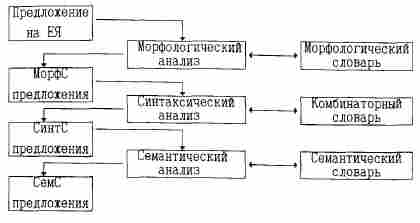
\includegraphics[scale=0.75]{scheme_l7p25}
	\end{itemize}

	\item Охарактеризуйте понятие лексемы.\hfill\\
	Слово в \textbf{широком} смысле -- единица морфологического анализа, единица толкового словаря, каноническая, основная, начальная форма словоформы (конкретной грамматической реализации слова). Объединяет собой все словоформы слова из словаря;Слово в \textbf{узком} смысле -- одинаковая последовательность фонем. Совокупность словоформ одной лексемы -- словоизменительная парадигма.

	\item Что такое морфема? аффикс? Какие виды аффиксов вы знаете?\hfill\\
	Элемент внутренней стркутуры слова. Мрофы: корневой, служебный (аффикс). Аффикс: префикс (приставка), суффикс, флексия(окончание) и постфикс. Аффикс носит дополнительный смысл. Проблема выделения аффиксов в составных слов.

	\item Чем основа слова отличается от корня? Приведите примеры.\hfill\\ \begin{itemize}
		\item Корневой морф -- это носитель основного смысла слова.
		\item Основа слова все морфы слова кроме флексий. Псведооснова -- неизменяемая часть слова. (л5 с12)
	\end{itemize}

	\item Что такое словоизменительная парадигма?\hfill\\
	Эта система изменений слова до словоформ. Слова могут изменяться без морфем (фонетически; супплетивно; сокращение безударных слов). Выделяет из всех словоформ слова инвариант (корень, основа) и перечень изменяемых компонентов (флективный класс окончаний, флексий; л5 с15). \textbf{Словоизменительный класс} -- набор всех слов с совпадающей морфологической парадигмой.

	\item В чем заключается лемматизация?\hfill\\
	Лемма -- словарная каноническая форма слова, слово в широком смысле. Лемматизация (нормализация) установление связи словоформы с её инвариантом -- словом (= лексемой). Стемминг -- приведение словоформы к (псевдо-) основе с требованием корректности в рамках словоизменительной парадигмы.

	\item Назовите основные стратегии морфологического анализа.\hfill\\
	Цель определение всех морфологических параметров словоформы и приведение её к лемме (или основе).
	Стратегии: \begin{itemize}
		\item словарный -- полный поиск по словарю с морфопарадигмами (большой объём) или по словарю (псевдо) основ (отдельный кеш существенных/неизменяемых слов, прочие: разделение на основу и флексию -> проверка соответствия флективного класса основы и флексии);
		\item статистический -- тегирование на машинным обучением с определённой оценко ошибки; инварианты слов встерчаются реже, чем аффиксы.
		\item неизвестные слова -- предсказание по префиксу или по финали? затем разбор по парадигме известной найденной словоформы.
		\item бессловарный -- определение морфологически характеристик (параметров) по псевдоокончаниям (последним буквам слов);
	\end{itemize}

	\item Приведите пример морфологической омонимии.\hfill\\
		стих, три, saw, left (не то но plane, lie, duck, bear)\\
		\url{http://www.really-learn-english.com/what-are-homonyms.html}

	\item Что такое синтаксическое дерево?\hfill\\ \begin{itemize}
		\item Отвечает на центральный вопрос синтакса -- структура предложения, связи между словами и их роли;
		\item Дерево -- это структура предложения с ролями составляющих его единиц, основанная на теории частей речи, и на предположении, что предложение выражает законченную мысль;
		\item Выделяет синтактические единицы: сказуемое, подлежащее, определение и дополнение. Строится на результате (пост-)морфологического анализа;
	\end{itemize}

	\item В чем особенность деревьев составляющих? Приведите пример.\hfill\\
	Выражает композиционную связь составляющих линейных отрезков текста (групп соседних слов, словосочетаний), причём пересечение недопустимо, но вложение допустимо. Само дерево -- иерархия вложений составляющих от частных слов (узлов-листьев) до всего предложения (агломеративное построение). Позволяетс составить грамматику, порождающую поредложение (терминалы -- слова, нетерминалы -- тпиы фраз, словосочетаний).\hfill\\
	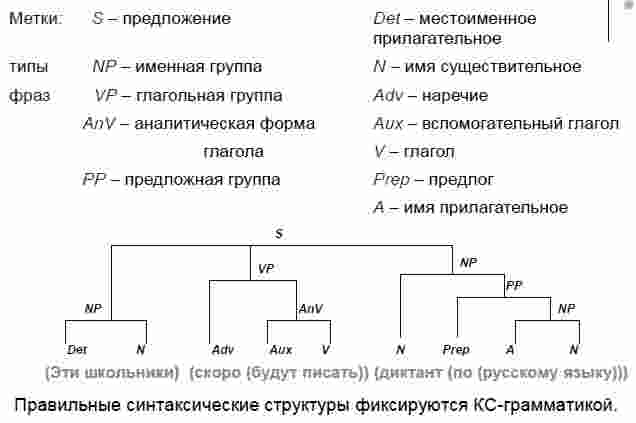
\includegraphics[scale=0.5]{constituent_tree}

	\item В чем особенность деревьев зависимостей? Приведите пример.\hfill\\
	Иерархия подчинительных связей главный-второстепенный (актант-сирконстант). Корень дерева -- глагол, узлы -- члены предложения, дуги дерева -- подчинительная связь. Определения подчиняются актантам/сирконстантам. Примеры типов связей: определительное, прямообъектное, сочинительное. (prep -> np)\hfill\\
	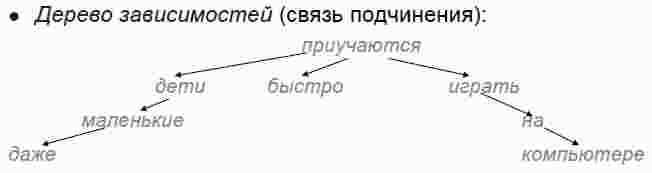
\includegraphics[scale=0.5]{subordination_tree}

	\item Чем проективное предложение ЕЯ отличается от непроективного?\hfill\\
	Рассматривается предложение как набор подчинительных связей между членами (словоформами). Проективность $\forall \alpha, \beta, \gamma \in S$ таких что $\alpha\to \beta$ ($\beta$ подчиняется $\alpha$) и в предложении $\gamma$ стоит между $\alpha$ и $\beta$, то $\alpha\to\gamma$. Человеческим языком: проективность -- дуги дерева не прерсекаются и не перескакивают корень дерева (сказуемое) (это условие не требуется в слабой проективности).

	\item Что такое валентность? Актант? Приведите примеры.\hfill\\
	Валентность -- свойство слова присединять другие единцы определённым способом (как арность предиката). Актант -- словосочетание, заполняющее ячейку валентности (объект, субъект), сирконстанты -- необязательные валентности слов-предикатов (обстоятельства). Имеются морфологические требования к актантам (падеж). Семантико-синтаксическая модель управления (л6 с41).\hfill\\
	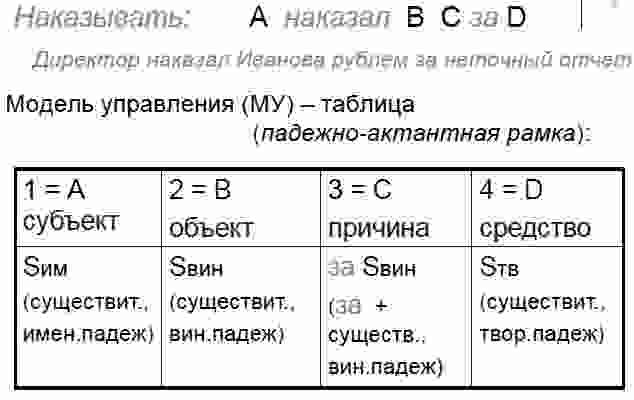
\includegraphics[scale=0.5]{valency}

	\item Какие методы и алгоритмы анализа контекстно-свободных языков вы знаете?\hfill\\
	(л7 с12) Нисходящие, восходящие, недетерминированные с возвратами. \begin{itemize}
		\item рекурсивный спуск (дерево рекурсивных вызовов функций на основе грамматики), алгоритм Эрли (сверху вниз), Кока-Янгера-Касами (разбор сверху вниз, КС грамматики A->BC, A->$\gamma$)
		\item Разрешение синтаксической омонимии состоит в построени нескоьких деревьев разбора и выборе наиболее вероятного по правилам грамматики согласно корпусу.
	\end{itemize}

	\item В чем состоит синтаксическая сегментация текста?\hfill\\
	\textbf{Предсинтаксический уровень} Разбиение текста на предложения, выделение простых предложений в составе сложных, разбиение предложений на составляющие локальные синтаксические группы на базе высоковероятных связей. (для определения л6 с18)

	\item Какие синтаксические типы словосочетаний вы знаете?\hfill\\
	Словосочетание -- это синтаксическая конструкция из знаменательных слов. Коллокация -- устойчиво (частотно) встречающееся словосочетание. Связи: Глагол - дополнение, сказуемое - подлежащее, существительное - дополнение, определяемое-определение л9 с14.

	\item В чем заключается закон Ципфа-Мальдельброта?\hfill\\
	частота появления слова обратно пропорциональна рангу этого слова по частоте (wut?) Неудивительно: любая величина обратно ``пропроциональна'' антимонотонному преобразованю самой себя. Идея в том, что частое слово используется часто, а редкое редко и частоты подчинятются степенному закону. \begin{itemize}
		\item ципф $f_i\sim \frac{1}{i}$;
		\item ципф-кондон $f_i\sim \frac{1}{i^a}$;
		\item ципф-мандельброт $f_i\sim \frac{1}{(i+n)^a}$ (это закон не языка а текста);
		\item Закон Хипса -- количество уникальных слов насызается с ростом объёма текста.
	\end{itemize}

	\item Какие статистические характеристики рассчитываются в статистических моделях?\hfill\\
	частоты единиц (различных словоупотреблений, словофром, слов, лексем); на их основе меры ассоциации; затем ранжирование

	\item Объясните понятие устойчивого словосочетания.\hfill\\
	Это словосочетание (коллокация слов), которое встречается в текстах или речи достаточно часто (устоявшееся выражение). Методы извлечения -- статистические (по частоте словесных n-грамм) или лингвистические (по синтаксическим образцам).

	\item Что такое мера взаимной информации Mutual Information?\hfill\\
	\item Какие статистические меры применяются для извлечения коллокаций?\hfill\\
	Нулевая гипотеза слова в словосочетании незавимимы -- сравнить фактическую частоту с предполагаемой. Меры ассоциации: \begin{itemize}
		\item \eng{(z-)t-score} (л6 с20) -- чем выше, тем меньше свидетельств в пользу гипотезы случайного сочетания слов;
		\item \eng{mutual information} (л9 с17) -- $\log_2 \frac{ \frac{f_{ab}^k}{N}}{ \frac{f_a}{N}\frac{f_b}{N}}$ где $k = 1$ или $3$ (для занижения значимости редких словосочетаний);  
		\item \eng{log-likelihood} (л6 с22) -- логарифм отношений правдоподобия -- сумма значений похожих на mutual information но не по парам слов, а по парам есть/нет слова (независимая биномиальная модель пары против ``зависимой'')
		\item \eng{dice} (л6 с24) -- доля от количества совместного появления от незавимсого появления составляющих.
	\end{itemize}

	\item Назовите отличительные характеристики связного текста.\hfill\\
	В связном тексте существуут коммуникативная преемственность между его составляющими. Каждое предложение в коммуникативном плане связано с предшествующим и продвигает высказывание от известного к новому, от данного, исходного к ядру.
	\url{http://www.hi-edu.ru/e-books/xbook029/01/part-005.htm}

	\item Что такое анафорическая ссылка?\hfill\\
	Ссылка на что-то, упомянутое ранее. Анафорическое слово или анафорическая ссылка соотносятся с антецедентом -- другими словом или предложением.

	\item Поясните понятие сверхфразового единства.\hfill\\
	семантико-синтаксическая единица текста, представляющая собой объединенность (тематическую и структурную) двух и более высказываний или фраз. Переход от одной темы к другой прорждает границу сверхфразовых единств. В связном тексте образуют тамтически-рематическую цепь (тема - данное, исходное; рема - новое, искомое);
	\url{http://www.hi-edu.ru/e-books/xbook029/01/part-005.htm}

	\item Объясните понятие лексической цепочки. Приведите примеры.\hfill\\
	порядка слов связаны именно с тема-рематическим строением высказывания, в частности при текстообразовании большую роль выполняют рематические компоненты вследствие того, что позиция ремы оказывается маркированной - это конечная позиция высказывания.

	\item Что такое тематическая структура текстов? Риторическая структура?\hfill\\
	\item Укажите принципы автоматического разрешения референции.\hfill\\
	\item Какие модели семантики текста вы знаете?\hfill\\
	Модель семантики предпочтения
	Модель концептуальной зависимости
	Модель «смысл - текст»

	\item В чем состоит задача разметки семантических ролей?\hfill\\
	определение семантических аргументов связанных с пердикатом или глаголом предложения и их классификация по специфичным ролям, отражающим общие свойства этого аргумента в описываемой предикатом ситуации. Позволяет выявить сходство в моделях управления различных предикативных слов. Следующий уровень абстракции после синтаксического дерева.	Неполный список ролей (Wikipedia), между которыми, правда, границы не всегда чёткие: \begin{description}
		\item[агенс] одушевлённый инициатор и контролёр действия;
		\item[пациенс] участник, претерпевающий существенные изменения;
		\item[бенефактив] участник, чьи интересы затронуты в процессе осуществления ситуации (получает пользу или вред);
		\item[экспериенцер] носитель чувств и восприятий;
		\item[стимул] источник восприятий;
		\item[] инструмент осуществления действия;
		\item[адресат] получатель сообщения (может объединяться с бенефактивом);
		\item[источник] исходный пункт движения;
		\item[цель] конечный пункт движения.
	\end{description} 

	\item Что такое термин? Приведите примеры.\hfill\\
	Термин -- слова и словосочетания, называющие понятия предметной области;

	\item Назовите основные свойства терминов.\hfill\\
	Грамматически паттерн AN или NN, чаще всего именные словосочетания (могут быть глаголы или наречия),

	\item Какие свойства родовидовых (таксономических) отношений вы знаете?\hfill\\
	\item Укажите принципы установления родовидовых (таксономических) отношений.\hfill\\
	\item Какие подвиды отношения часть-целое вы можете назвать?\hfill\\

	\item Какие отличительные признаки корпуса текстов вы можете назвать?\hfill\\
	сильно зависит от задачи: сбалансированность, репрезентативность, размеченность.

	\item Что такое параллельный и псевдопараллельный корпус?\hfill\\
	Мультиязыковой корпус текст+перевод и всё с разметкой.

	\item Назовите и охарактеризуйте типичные приложения компьютерной лингвистики.\hfill\\
	\item В чем особенности задачи извлечения информации из текстов?\hfill\\
	\item Укажите основные стратегии машинного перевода. Что такое интерлингва?\hfill\\
	\item В каких прикладных задачах применяется генерация текста?\hfill\\
	\begin{itemize}
		\item машинный перевод -- пословный перевод, пословно-пооборотный (приемлимое качество для родственных), пофразный, использование языка-посредника, статистическая трансляция;
		\item информационный поиск -- нахождение релевантных документов по ключевым словам или запросу; индексирование документа для выделения ключевых слов; для классификации, рубрицирования, создания подмножеств схожих документов, аннотирования (сжатое описание) или реферирования (краткое реферат нескольких текстов);
		\item вопросно-ответные системы;
		\item синтез текста по информации в нетекстовой форме;
		\item извлечение информации -- распознавание объектов, связей, субъектов, событий и фактов на основе предсинтаксичесокго анализа или лингвистических шаблонов;
		\item определение тональности -- извлечение, анализ и классификация мнений или суждений;
		\item проврека орфографии, коррекция текстов, расстановка переносов, вычисление и исправление паронимнических ошибок (неправильное использование).
	\end{itemize}

	\item Охарактеризуйте понятие лингвистического шаблона.\hfill\\
	Это упорядоченное множество шаблонов поиска слов (троек лексема, часть речи морфологические параметры). По сути это синтаксический шаблон с лексическими и морфологическими критериями.
\end{enumerate}

Вопросы:
\begin{enumerate}
	\item Что является результатом полного морфологического анализа словоформы? Поясните на примере конкретной словоформы.
	\item В чем отличие синтаксических деревьев непосредственно составляющих от синтаксических деревьев зависимостей?
	\item Что такое непроективность предложения? Слабая непроективность? Привести собственные примеры.
	\item Что такое валентность? Актант? Слово-предикат? Проиллюстрировать на примере.
	\item Какие бывают виды сегментации текста? Охарактеризуйте синтаксическую сегментацию.
	\item Укажите типы лексических отношений.\hfill\\
	Избирательность лексем; Идиоматичность словосочетаний (л6 с33)

	\item Что такое семантические классы слов?\hfill\\
	Объединение слов одной части речи в группу с общим основным компонентом значения (температурные прилагательные); тематический класс -- объединине слов на основе совпадения тематики основного смысла (категория названия видов живых организмов).

	\item Охарактеризуйте особенности описания семантических ролей в проекте FrameNet.\hfill\\
	\eng{Frame} -- схематическое прдтавление ситуации с участниками и ролями. Выделяются основные (действие-объект-субъект) и вспомогательные элементы (обстоятельства), которые являющиеся синтаксическими единицами в конкретном предложении. Учитываются связи между фреймами: \begin{description}
		\item [Наследование] Отношение уточнения или (обратной абстракции): что справедливо для родителя, считается справедливым для наследника;
		\item [Перспектива] Нейтральный фрейм относится к фрейму, указывающему на ``направленность'' ситуации: передача товара - \textbf{покупатель} или \textbf{продавец};
		\item [Субфрейм] Композиция фреймов, содержащих сложные сценарии: ``судебный процесс'' связан со многими подсценариями, состояниями и событиями;
		\item [Предшествование] Определяет временной порядок между субфреймами сложного сценария;
		\item [Причинно-следственная]
		\item [Использование] Сценарий одного фрейма косвенным образом затрагивает другой фрейм: ``вынесение суждения'' использует, но не наследует от фреймов ``суждение'' или ``утверждение'';
	\end{description}

	\item Какие психолингвистические предположения легли в основу создания WordNet?\hfill\\
	основное отношение между словами -- синонимия. Синонимичные слова отражают почти идентичную концепцию, и во многих контекствах могут быть взаимозаменяемыми. Слова сбиваются в \eng{Synset}'ы по синонимии, однако это \textbf{не} классы эквивалентности. Между \textbf{Синсетами} существуют немногочисленные ``концептуальные отношения''. Виды отношений основаны на результатах психолингвистических исследований 60-х годов. \begin{description}
		\item[вложение] или \eng{hyperonymy}, \eng{hyponymy} задаёт транзитивное отношение на смыслах синсетов от общего к частному. Синсеты существительных в конечно итоге объединены под корневым \eng{synset} узлом ``сущность''. Для существительных выделяются промежуточные узлы \textbf{типы} (имена нарицательные) и листья \textbf{реализации} (имена собственные, термины, названия). Для глаголов это уточнение манер и оттенков действия или события (\emph{общаться}-\emph{разговаривать}-\emph{шептать}). 
		\item[составная часть] \eng{meronymy} задаёт отношение часть-целое (\emph{ножка}-\emph{стул} или \emph{держало}, \emph{хлебало}-\emph{ложка}). Части наследуются вниз по вложению, от общего к частному, но не наоборот.
		\item[полярность] или антонимия, отношение отражающее прямой контраст между элментами синсетов прилагательных;
		\item[сходство] смысловая ``похожесть'' прилагательных; 
	\end{description}
	\url{http://www.cl.ut.ee/yllitised/viderorav.html}


	\item Что такое лингвистические онтологии? В чем их особенность?\hfill\\
	\item Назовите классы словосочетаний по степени фразеологичности, приведите примеры.\hfill\\

	\item Укажите лингвистические критерии извлечения коллокаций.\hfill\\
	Грамматические (образцы), лексические (списки слов и словосочетаний), контектстные (окружени термина в тексте)

	\item Что такое мера ассоциации? Для чего применяются меры? Приведите примеры мер.

	\item Укажите формулу подсчета и особенности применения меры Mutual Information для извлечения коллокаций.

	\item Статистический машинный перевод: особенности технологии.\hfill\\

	\item Особенности задачи автоматической генерации текстов, этапы генерации.\hfill\\
\end{enumerate}

Задачи:
\begin{enumerate}
	\item Для заданной фразы построить возможные синтаксические деревья зависимостей.
	\item Составить семантико-синтаксическую модель управления заданного слова.
\end{enumerate}



% section review (end)

\end{document}

